
\section{Ohm's Law}

Name \rule{2.0in}{0.1pt}\hfill{}Section \rule{1.0in}{0.1pt}\hfill{}Date
\rule{1.0in}{0.1pt}

\textbf{Objectives}

\begin{itemize}
\item To investigate the most important principle in electronics.
\item To determine how resistors in series and parallel add.
\end{itemize}
\textbf{Introduction}

The rate at which electric charge flows through a conductor is called
the electric current. In order to have a current, a potential difference,
or voltage is necessary. We first want to determine the relationship
between the potential difference at two ends of a conductor and the
current flowing through it.

\textbf{Note}: Do not turn on a power supply until you are sure your
circuit is correct. If you are at all unsure, please ask your instructor
to approve your setup. Ammeters can be instantly and permanently ruined
by an improper connection. Be sure to turn off the power supply before
making any changes to the circuit.

\textbf{Apparatus}

\begin{itemize}
\item power supply
\item 2 rheostats
\item ammeter
\item voltmeter
\end{itemize}
\textbf{Activity 1: Ohm's Law}

\begin{itemize}
\item Connect two rheostats (or variable resistors) in series as shown in
the figure below. Set R\( _{1} \) at about the halfway point and
R\( _{2} \) at the maximum. Connect an ammeter as shown. Also, connect
a voltmeter across (that is, connect a probe to each side of) R\( _{1} \).
\end{itemize}
\vspace{0.3cm}
{\centering \resizebox*{0.35\textwidth}{!}{\includegraphics{ohms_law_fig_1.eps}} \par}
\vspace{0.3cm}

\begin{itemize}
\item When sure of your circuit, turn on the power supply, and turn
the voltage up all the way..
\item Record the current through the circuit and the voltage across R\( _{1} \).\vspace{10mm}

\item Reduce the resistance of R\( _{2} \) and record the current and voltage
three more times by turning down the rheostat in approximately equal
steps so that for the last time R\( _{2} \) is turned completely down.\vspace{30mm}

\item Turn off the power supply.
\item Plot your four pairs of readings with the voltage on the vertical axis
and the current on the horizontal axis.
\item Fit a straight line to the points, using the origin as a fifth point.
\item Is a straight line a good fit to the data? What does that say about
the relationship between voltage and current?\vspace{15mm}

\item What are the value and meaning of the slope of this line? Write the
equation of the line.\vspace{15mm}

\item Remove R\( _{1} \) from the rest of the circuit and use the ohmmeter
option on the multimeter to measure the resistance of R\( _{1} \).
Does it agree with the slope you found? What is the percent difference?
Replace R\( _{1} \).\vspace{30mm}

\item What is the general relationship between voltage, current, and resistance?
This is Ohm's Law.\vspace{15mm}

\item Why is the origin a legitimate point on the curve?\vspace{15mm}

\end{itemize}
\textbf{Activity 2: Resistors in Series}

\begin{itemize}
\item Turn rheostat R\( _{2} \) to its maximum setting. Connect the multimeter
across this resistor, being sure to set it for reading voltages.
\item When you are sure the circuit is set, turn on the power supply and
record the current and voltage. Turn off the power supply.\vspace{10mm}

\item \textbf{Prediction}: Based on your measurements, predict the resistance
of R\( _{2} \).\vspace{15mm}

\item Remove and measure the resistance of R\( _{2} \). Record the percent
difference between your prediction and measurement. Replace R\( _{2} \).\vspace{30mm}

\item Was the current this time different from the first reading in Activity
1?\vspace{15mm}

\item What can you conclude about the current through two resistors in series?\vspace{15mm}

\item Connect the multimeter across both resistors, being sure to switch
to voltage readout.
\item When you are sure the circuit is correct, turn on the power supply
and record the current and voltage. Turn off the power supply.\vspace{10mm}

\item Has the current changed?\vspace{15mm}

\item Has your previous conclusion been substantiated or refuted?\vspace{15mm}

\item How is the voltage just measured related to the first voltage measurements
in Activities 1 and 2?\vspace{15mm}

\item What can you conclude about the voltage across resistors in series?\vspace{15mm}

\item Using your conclusions concerning voltages across and current through
resistors in series and your formulation of Ohm's law, what can you
conclude about the total resistance in a circuit having two resistors
in series?\vspace{15mm}

\end{itemize}
\textbf{Activity 3: Resistors in Parallel}

\begin{itemize}
\item Connect the two rheostats in parallel as shown in the figure below,
with the ammeter at the point marked A and the voltmeter across the
two rheostats. Set the rheostats at about their halfway settings.
\end{itemize}
\vspace{0.3cm}
{\centering \resizebox*{0.35\textwidth}{!}{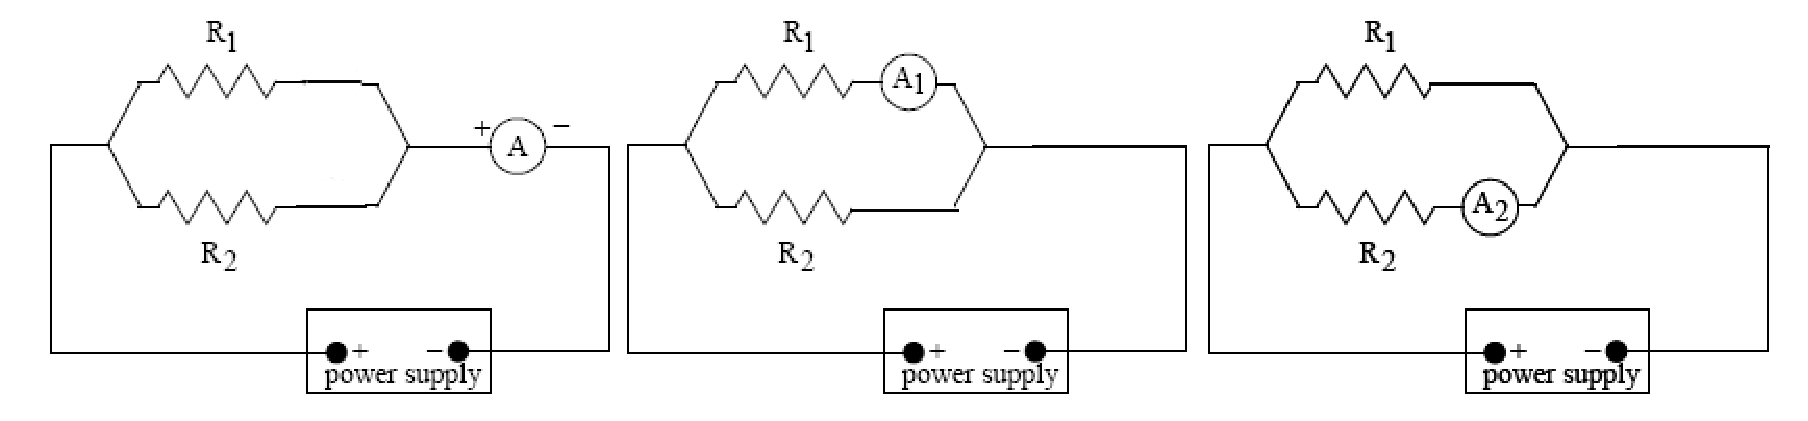
\includegraphics{ohms_law_fig_2.eps}} \par}
\vspace{0.3cm}

\begin{itemize}
\item When you are sure the circuit is set up correctly, turn on the power
supply and record the total current through the circuit and the voltage
drop across the parallel resistance combination. Turn off the power
supply.\vspace{10mm}

\item Connect the ammeter to the point marked A\( _{1} \) without disturbing
the rest of the circuit; apply power and record the current through
R\( _{1} \) and the voltage reading. Turn off the power supply.\vspace{10mm}

\item Repeat the above measurements for R\( _{2} \), connecting the ammeter
at A\( _{2} \) instead of A\( _{1} \).\vspace{10mm}

\item Using Ohm's Law, calculate the two resistances of the parallel connection
and also the total resistance of the circuit. Check with the ohmmeter
and determine the percent differences.\vspace{30mm}

\item What is the relationship between the total current and the current
in each of the branches of the parallel circuit?\vspace{15mm}

\item What is the relationship between the total resistance of the parallel
circuit and the resistance of each of the branches (you may want to
look up in a reference what the correct relationship should be and
see if your result agrees with it)?\vspace{15mm}

\item Determine, using Ohm's law, what the voltage was in each branch of
the parallel circuit. Did it make any difference that you didn't reposition
the voltmeter during this activity? On the basis of Ohm's law, does
the result make sense?\vspace{30mm}

\item Can the total resistance of a series combination ever be less than
the resistance of the largest resistor? Explain.\vspace{30mm}

\item Can the total resistance of a parallel combination ever be greater
than the resistance of the smallest resistor? Explain.\vspace{30mm}
\end{itemize}

